% !TEX root=exama-221129-orap.tex
%--------------------------------------
% Create title frame
\titleframe

%--------------------------------------
% Table of contents
\begin{frame}{Overview}
  \setbeamertemplate{section in toc}[sections numbered]
  \tableofcontents[hideallsubsections]
\end{frame}


%==============================================
\section{Exa-MA: Methods and Algorithms at Exascale}

\subsection{Exa-MA}

\begin{frame}
  \frametitle{Objectives}

  \begin{center}
    \Large Scale up methods and algorithms in predictive simulation data analysis, up to digital twinning, including uncertainty quantification and inverse problems
  \end{center}

  \begin{itemize}
    \item Produce methods and algorithms 
    \item Produce patterns
    \item Produce software
    \item Produce benchmarks
  \end{itemize}
\end{frame}

\subsection{Challenges}
\begin{frame}
  \frametitle{\insertsectionhead}
  \framesubtitle{\insertsubsectionhead}
  \footnotesize
  \begin{columns}
    \column{.5\textwidth}
    \begin{itemize}
      \item (C1) Reduce carbon (GHG) footprint in transportation, buildings, and cities
       \item (C2) Design, control, and manufacture of advanced materials
       \item (C3) Understand and simulate the human brain
       \item (C4) Understand fission and fusion reactions and design advanced experiment facilities for fusion
             \end{itemize} 
    \column{.5\textwidth}
    \begin{itemize}
      \item (C5) Monitor the health of our planet: climate prediction, impact assessment of environmental policies, rapid environmental hazards

        \item (C6) Monitor and personalize the health of human beings 
       \item (C7) Design drugs
       \item (C8) Design cost-effective renewable energy resources: batteries, biofuels, solar photovoltaics
       \item (C9) Understand the Universe
     \end{itemize} 
  \end{columns}

\end{frame}
\subsection{Bottlenecks}
\begin{frame}[fragile=singleslide]{\insertsectionhead}
  \framesubtitle{\insertsubsectionhead}
  \scriptsize
  \begin{columns}[]
    \begin{column}{.5\linewidth}
      \begin{itemize}
        \item (B1) Energy efficiency
        \item (B2) Interconnect Technology
        \item (B3) Memory technology
        \item (B4) Scalable systems software
        \item (B5) Programming systems
        \item (B6) Data Management
        \item (B7) Exascale Algorithms
      \end{itemize}
    \end{column}
    \begin{column}{.5\linewidth}
      \begin{itemize}
        \item (B8) Discovery, design, and decision algorithms
        \item (B9) Resilience, robustness and accuracy
        \item (B10) Scientific productivity
        \item (B11) Reproducibility, replicability of computation
        \item (B12) Pre/Post-processing
        \item (B13) Integrate Uncertainties
      \end{itemize}
    \end{column}
  \end{columns}
  \begin{alertblock}{Major Concerns}
    \footnotesize
    \begin{itemize}
      \item avoidance of communication  
      \item adaptive parallel grain and more compute-intensive at node level 
      \item handling of heterogeneous hardware and data representations and 
      \item self parametrization
    \end{itemize}
  \end{alertblock}
  
\end{frame}

\begin{frame}
  \frametitle{Exa-MA is a Part of the NumPEx Software Stack}

  \begin{columns}[]
    \begin{column}{.5\linewidth}
      \begin{center}
        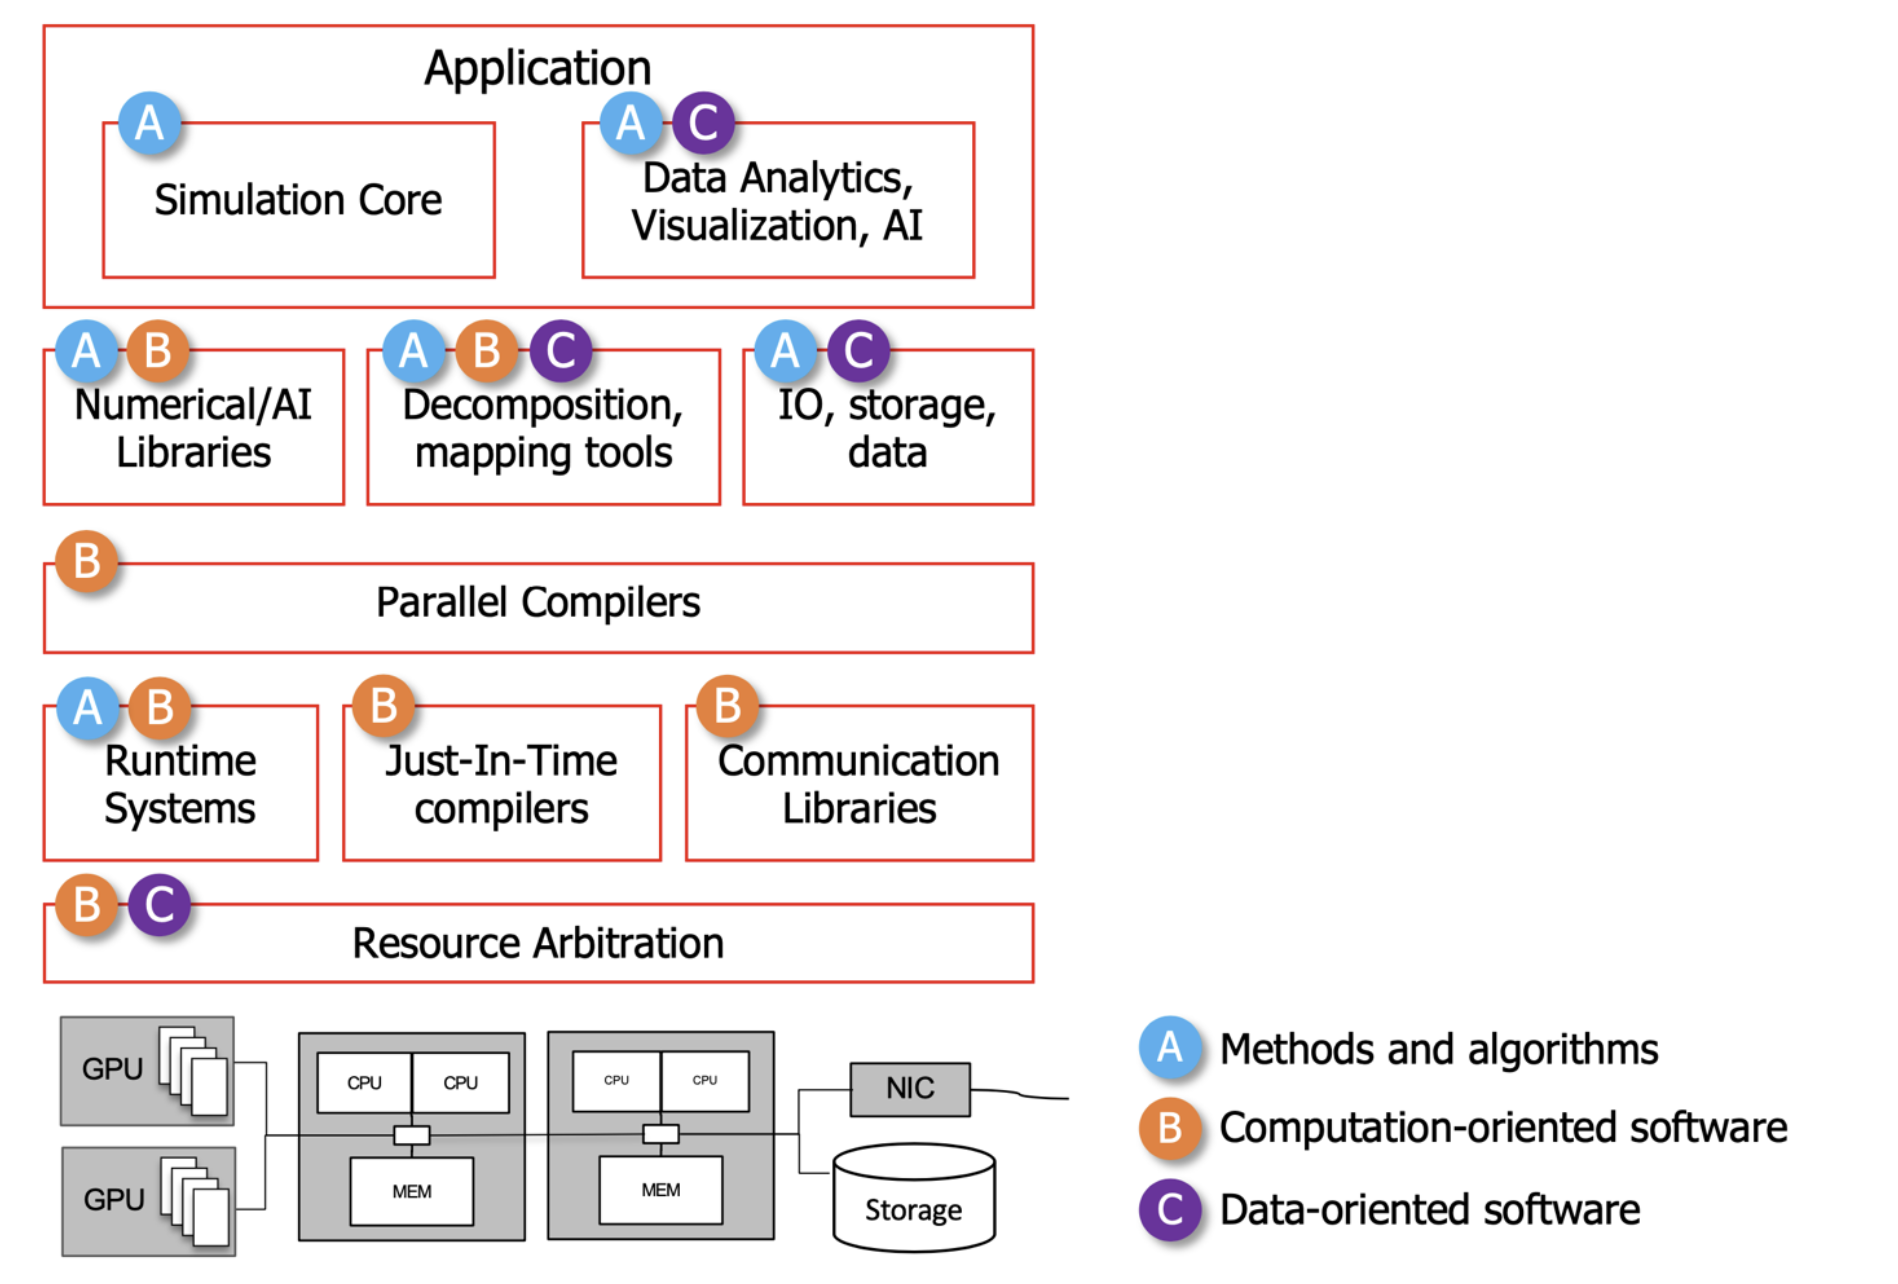
\includegraphics[height=.8\textheight]{../../figures/software-stack.png}  
      \end{center}
    \end{column}
    \begin{column}{.5\linewidth}
      Enable
      \begin{itemize}
        \item Performance and Scalability
        \item Productivity
        \item Reproducibility and reusability
        \item Efficiency, resilience, robustness
      \end{itemize}
    \end{column}
  \end{columns}
  
  
\end{frame}
\section{Work Packages}
\subsection{WP1: Discretization}
\begin{frame}
  \frametitle{\insertsectionhead}
  \framesubtitle{\insertsubsectionhead}

  \begin{columns}[t]
    \column{.5\textwidth}
    Objectives
    \begin{itemize}
      \item Geometric domain representations and their discrete counterparts 
      \item Physics-based models 
    \end{itemize}
    Specifications
    \begin{itemize}
      \item Favor high order methods to increase local compute load
      \item Favor non-conforming methods to reduce communication
    \end{itemize}
    \begin{alertblock}{Links}
      PC2-WP2/3, PC3-WP3 
    \end{alertblock}
    \column{.5\textwidth}
    Tasks
    \begin{itemize}
      \item Geometric representation and their discrete counterparts  including valid mesh generation and adaptive mesh refinement (AMR) 
      \item Space-Time Discretization of PDEs leveraging non-conforming methods and AMR as well as parallel in time methods
      \item Multi-Physics and Multiscale coupling[B7, B10] 
    \end{itemize}


  \end{columns}
\end{frame}


\subsection{WP2: Reduced order and AI driven methods for multi-fidelity modeling} 
\begin{frame}
  \frametitle{\insertsectionhead}
  \framesubtitle{\insertsubsectionhead}
\footnotesize
  \begin{columns}[t]
    \column{.5\textwidth}
    Objectives
    \begin{itemize}
      \item Develop Reduced order methods 
      \item Develop methods for multi-fidelity modeling 
    \end{itemize}

      Specifications
      \begin{itemize}
        \item Leverage beyond state of the art reduce order, surrogate and machine learning methods
        \item Enable Multi-fidelity modeling
      \end{itemize}
    \column{.5\textwidth}
    Tasks
    \begin{itemize}
      \item surrogate models based on physics driven deep learning
      \item PDE operator learning using NN
      \item data driven model order reduction
      \item non-intrusive and weakly intrusive reduced basis methods for parametrized PDEs
      \item mixing low and high fidelity models
      \item real-time models with super resolution methods
    \end{itemize}
    \begin{alertblock}{Links}
      PC2-WP2/3, PC3-WP3
    \end{alertblock}

  \end{columns}
\end{frame}

\subsection{WP3: Linear, Multi-linear and Coupled Solvers at Exascale}
\begin{frame}
  \frametitle{\insertsectionhead}
  \framesubtitle{\insertsubsectionhead}
  \footnotesize
  \begin{columns}[t]
    \column{.5\textwidth}
    Objectives
    \begin{itemize}
      \item Focus on generic building blocks(algebraic) for informations
      \item Support high dimensional problems
    \end{itemize}
    Specifications: 
    \begin{itemize}
      \item Communication avoiding algorithms
      \item low-precision computing
      \item matrix-free methods
      \item operator/data compression
    \end{itemize}
    \column{.5\textwidth}
    Tasks
    \begin{itemize}
      \item Acceleration techniques for subspace-based methods;
      \item High dimensional problems ;
      \item Randomization;
      \item Exploiting data-sparsity and multiple precision;
      \item Adaptive solution strategies for exascale multiphysical and multiscale models;
    \end{itemize}
    \begin{alertblock}{Links}
    PC2-WP2/3   
  \end{alertblock}
  \end{columns}
\end{frame}

\subsection{WP4: Combine data and models, inverse problems at Exascale }
\begin{frame}
  \frametitle{\insertsectionhead}
  \framesubtitle{\insertsubsectionhead}
  \begin{columns}[t]
    \column{.5\textwidth}
    Objectives
    \begin{itemize}
      \item Improve existing deterministic methods 
      \item  Formulate new stochastic methods. 
      \item Improve observation strategies.
      \item Implement multi-fidelity schedules  
    \end{itemize}
    Specifications:
    \begin{itemize}
      \item combine model and data 
      \item Enable deterministic and stochastic methods
    \end{itemize}
    \column{.5\textwidth}
    Tasks
    \begin{itemize}
      \item Deterministic methods
      \item Stochastic methods
      \item Observations
      \item Taking advantage of multi-fidelity modeling
      \item Challenges of multi-fidelity in inverse problems: criteria to update reduced models.
    \end{itemize}
    \begin{alertblock}{Links}
    PC2-WP2/3,PC3-WP3
  \end{alertblock}
  \end{columns}
\end{frame}

\subsection{WP5: Optimize at Exascale }
\begin{frame}
  \frametitle{\insertsectionhead}
  \framesubtitle{\insertsubsectionhead}
  \begin{columns}
    \column{.5\textwidth}
    Objective: Design and implement of large scale optimization problems
    \begin{itemize}
      \item combinatorial continuous and mixed optimization
      \item surrogate-based optimization
      \item shape optimization 
    \end{itemize}
    \column{.5\textwidth}
    Specifications / Tasks
    \begin{itemize}
      \item Decomposition-based methods
      \item Learning-based methods, e.g. surrogate models and multi-fidelity representation
      \item Auto-tuning for ML
      \item Reduced order and ML for shape optimization 
    \end{itemize}
    \begin{alertblock}{Links}
      PC2-WP2/3,PC3-WP2 
    \end{alertblock}
  \end{columns}
\end{frame}

\subsection{WP6: Quantify uncertainty at Exascale}
\begin{frame}
  \frametitle{\insertsectionhead}
  \framesubtitle{\insertsubsectionhead}
  \footnotesize
  \begin{columns}
    \column{.5\textwidth}
    Objectives
    \begin{itemize}
      \item Sensitivity analysis for dimension reduction, ranking and more generally understanding the influence of uncertain input parameters.
       \item  Propagation of uncertainties
      \item Surrogate modeling for UQ
      \item Acceleration of the bricks of UQ process steps by leveraging exascale calculations
    \end{itemize}

    \begin{alertblock}{Links}
      PC2-WP2/3,PC3-WP2/3
    \end{alertblock}
    \column{.5\textwidth}
    Specifications / Tasks
      \begin{itemize}
        \item Extension of kernel methods to complex inputs/outputs
        \item global sentivitity analysis (GSA) 
        \item  GSA in the presence of uncontrollable stochastic random input
        \item Multi-scale GSA in code coupling/chaining
        \item GSA with complex input 
        \item  Links between kernel-based sensitivity indices (HSIC, MMD) and total Sobol indices
      \end{itemize}


  \end{columns}
\end{frame}

\subsection{WP7: Demonstrate methods and algorithms at Exascale}
\begin{frame}
  \frametitle{\insertsectionhead}
  \framesubtitle{\insertsubsectionhead}

  \begin{columns}
    \column{.5\textwidth}
    \begin{itemize}
      \item Benchmarking on small/mini apps 
      \item Showroom of methods and algorithms
      \item Co-design with the CDT and PC5
    \end{itemize}
    \column{.5\textwidth} 
    \begin{alertblock}{Links}
      PC2-WP2/3,PC3-WP2/3 and PC5
    \end{alertblock}
   
  \end{columns}
\end{frame}

\begin{frame}[plain]
  \frametitle{}
  \framesubtitle{}

  \begin{center}
    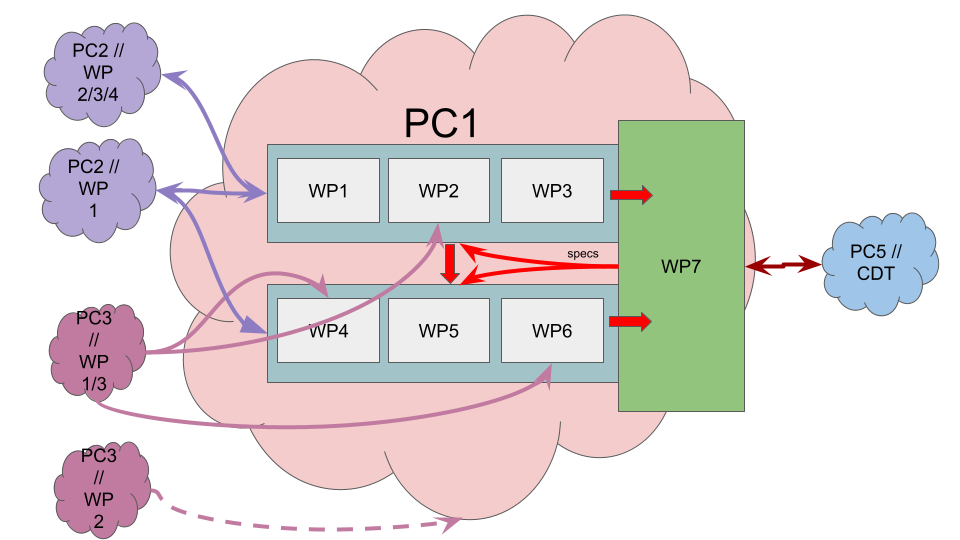
\includegraphics[width=.9\linewidth]{../../figures/exama-pc.png}
  \end{center}

  

\end{frame}

%\section{Deliverables}

\begin{frame}
  \frametitle{Deliverables}
  %\framesubtitle{\insertsubsectionhead}
\vspace*{-0.5cm}
  \begin{center}
    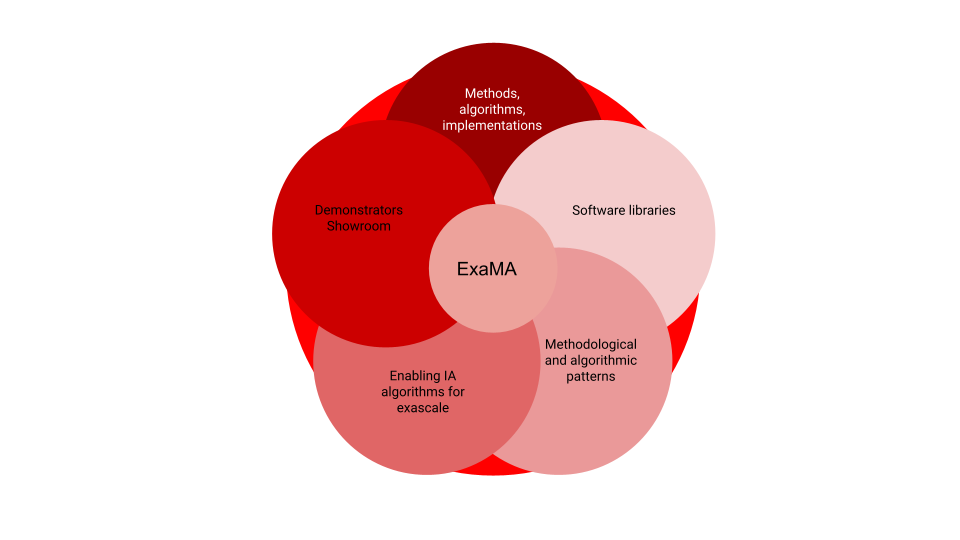
\includegraphics[width=\linewidth]{../../figures/exama-deliverables.png}
  \end{center}
  % \begin{itemize}
  %   \item  Methods, algorithms, and implementations that, taking advantage of the exascale architectures, empower modeling, solving, assimilating model and data, optimizing and quantifying uncertainty, at levels that are unreachable at present.
  %   \item Software libraries allowing to assemble specific critical reusable components, hiding the hardware complexity and exposing only the specific methodological interface
  %   \item Methodological and Algorithmic Patterns at exascale that can be reused efficiently in large scale applications (eg in weather forecasting)
  %   \item Enabling AI algorithms to attain performances at exascale, exploiting the methods (point 1) and the libraries (point 2) developed.
  %   \item \href{https://docs.google.com/document/d/1hjwSFRF63SyTUJJKGMNLHcJPr_S2JDHYXeBeQzHCSno/edit?usp=sharing}{\beamergotobutton{Demonstrators}}
% 
  % \end{itemize}


\end{frame}

% \subsection{Milestones}

\begin{frame}
  \frametitle{Milestones}
%  \framesubtitle{\insertsubsectionhead}
\vspace{-0.5cm}
  \begin{center}
    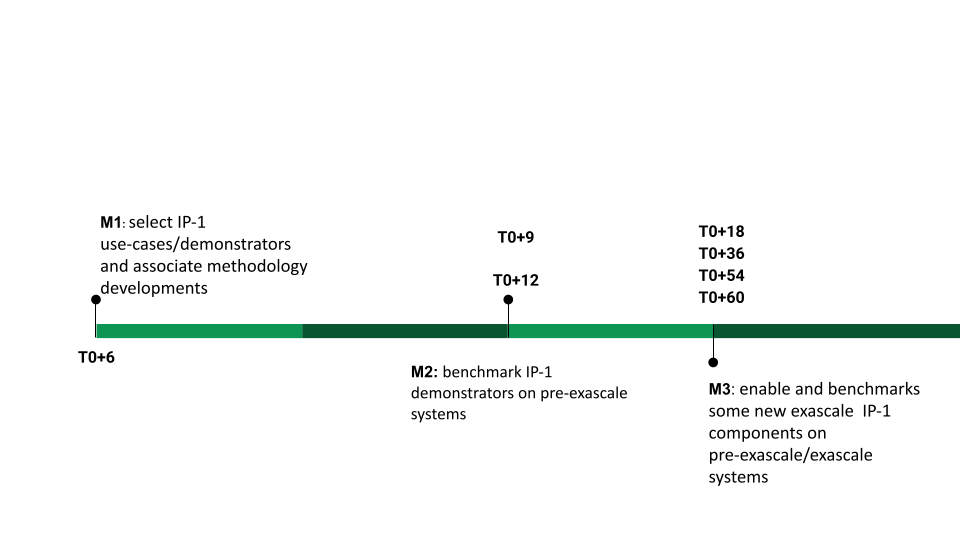
\includegraphics[width=\linewidth]{../../figures/exama-timeline.png}
  \end{center}


%   \begin{itemize}
%     \item   M1 Select IP-1 use-cases/demonstrators and associate methodology developments T0+6
%     \item M2 benchmark IP-1 demonstrators on pre-exascale systems T0+9/T0+12
%     \item M3 enable and benchmarks some new exascale  IP-1 components on pre-exascale/exascale systems T0+18, T0+36, T0+54, T0+60
% \end{itemize}


\end{frame}




\section{Relations}

\subsection*{External Partner Status}
\begin{frame}
  \frametitle{\insertsectionhead}
  \framesubtitle{\insertsubsectionhead}

  Setting up this network and creating a group of external partners, we will succeed in
  \begin{itemize}
    \item bringing together our community to solve scientific challenges to move to the Exascale
    \item jointly develop software bricks to scale up to exascale
    \item creating/strengthening collaborations between external partners and Exa-MA partners via project co-leads, co-funding and/or use cases
    \item better structuring our community to respond effectively to European and international calls for projects.
  \end{itemize}

\end{frame}
\subsection{Entreprises}
\begin{frame}
  \frametitle{\insertsectionhead}
  \framesubtitle{\insertsubsectionhead}
  \begin{alertblock}{Entreprises}
    \begin{itemize}
      \item Expected: EDF, Safran, TotalEnergies, Atos, Airbus
      \item Positive contact: Roche
    \end{itemize}
  \end{alertblock}
\end{frame}

\subsection{EPIC \& PEPR}
\begin{frame}
  \frametitle{\insertsectionhead}
  \framesubtitle{\insertsubsectionhead}
\begin{alertblock}{EPIC}
  \begin{itemize}
    \item Expected: Onera
    \item Positive contact: Ifpen
  \end{itemize}
\end{alertblock}

\begin{alertblock}{PEPR}
  \begin{itemize}
    \item Expected: IA
    \item Others: Diadem, TRACCS-Météo (in particular PC1-WP4)
  \end{itemize}
\end{alertblock}

\end{frame}

\subsection{Europe}
\begin{frame}
  \frametitle{\insertsectionhead}
  \framesubtitle{\insertsubsectionhead}
  \begin{alertblock}{CoE}
    \begin{itemize}
      \item Expected: Hidalgo2, Cheese-2P
      \item Others: CoE	EoCoE-3
    \end{itemize}
  \end{alertblock}

  \begin{alertblock}{Europe}
    \begin{itemize}
      \item Expected: ERC-Synergy WholeSun, ERC-Synergy	EMC2, EuroHPC	Microcard, EuroHPC	European Master for HPC - EUMaster4HPC	
      \item Others ?
    \end{itemize}
  \end{alertblock}
\end{frame}

\begin{frame}[plain]
  \frametitle{}
  \framesubtitle{}
\begin{center}
  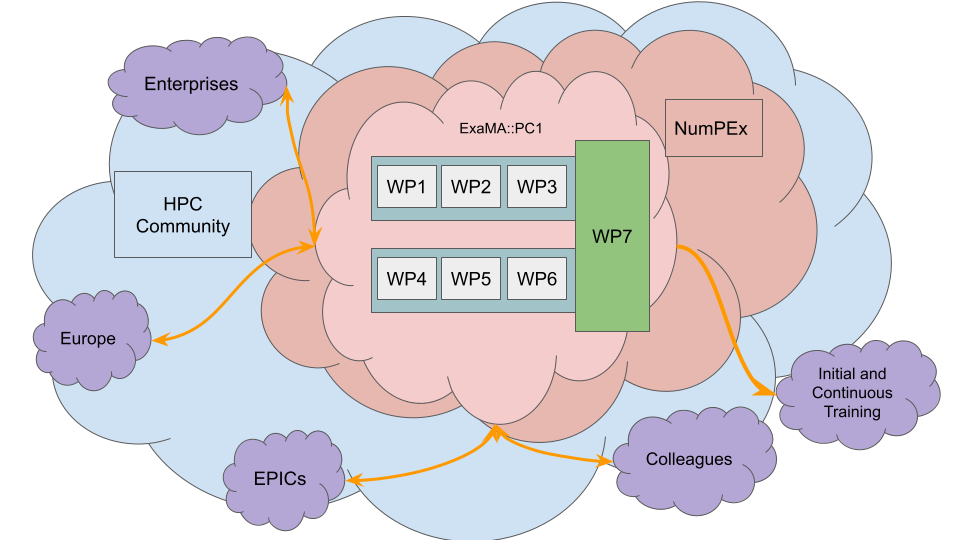
\includegraphics[width=.9\linewidth]{../../figures/exama-relations.png}
\end{center}
  
\end{frame}



\begin{frame}
  \frametitle{}
  \framesubtitle{}

  \begin{center}
    \LARGE We are building the Exa-MA community \\[1cm]

    Thank you for your attention!
  \end{center}
  
  

\end{frame}

\appendix
\section{Appendix}
%==============================================
%==============================================
\subsection{NumPEx::Exa-MA}

\begin{frame}
  \frametitle{\insertsectionhead}
  \framesubtitle{\insertsubsectionhead}

  Partners
  \begin{itemize}
    \item CEA 
    \item INRIA : Bordeaux,  Côte d'Azur, Grenoble, Lille, Paris, Saclay
    \item IPP 
    \item Sorbonne Université 
    \item UNISTRA  
  \end{itemize}
\end{frame}


